\setcounter{secnumdepth}{-1}

\chapter{Shika na Mikono Hands-On Activities}

\section{Shika Express Demonstrations for Physics}

\begin{multicols}{2}


\subsection{Data on Weighing}

\begin{center}
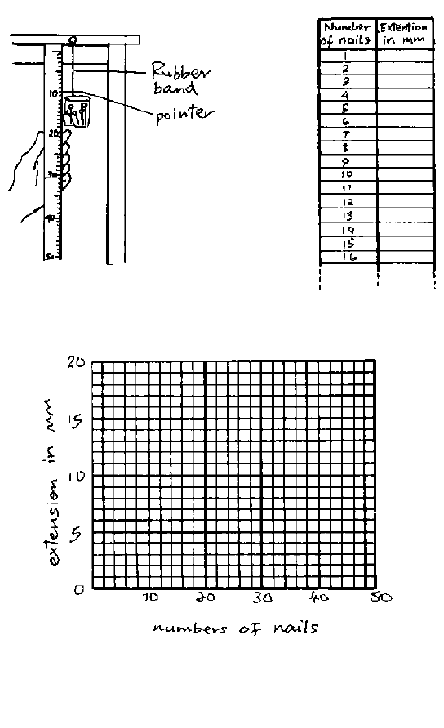
\includegraphics[width=0.4\textwidth]{./img/source/meas-mass.png}
\end{center}

Fix a rubber band at one end to a table or retort stand. At the other end, attach a paper clip to act as a pointer and a small bag or scale pan. Fill the bag or scale pan with successive numbers of nails. Have students measure the extension of the rubber band each time they add more nails. Record the readings and use the data to draw a graph as shown in the figure.

\subsection{Density Column}
\label{sub:density-column}

\begin{center}
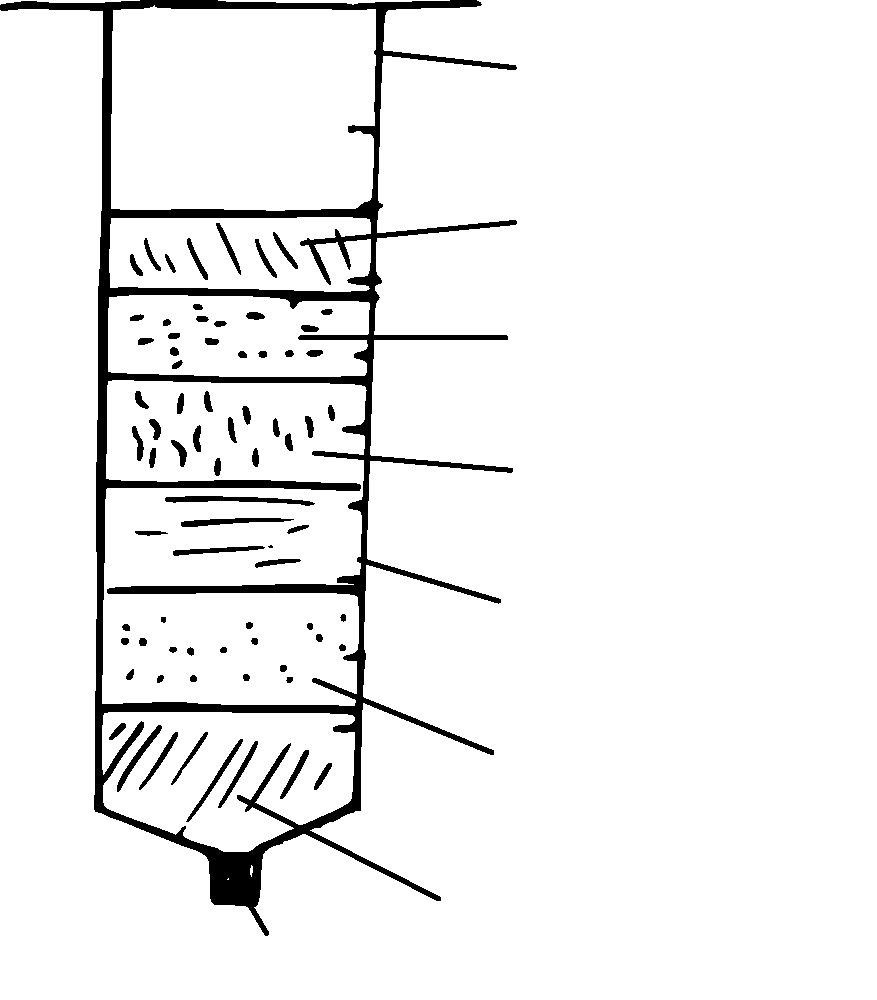
\includegraphics[width=0.25\textwidth]{./img/density-tower.png}
\end{center}

\begin{description*}
\item[Topic:]{Density - Form I}
\item[Materials:]{Syringes, water, honey, glycerine, cooking oil, spirit, kerosene, erasers, paper clips, nails, other small objects}
%\item[Setup:]{}
\item[Procedure:]{Add each liquid into the syringe, one by one, observing the relative depths of each liquid. Place small solid objects e.g. rubber erasers, paper clips, small nails, etc. into the syringe and observe their positions relative to the various liquids.}
%\item[Hazards:]{}
\item[Questions:]{Which liquid is the most dense? Which is the least dense?}
\item[Observations:]{The denser liquids sink to the bottom while the less dense liquids rise to the top. The solid objects settle among liquids of comparable density.}
\item[Theory:]{}
\item[Applications:]{Relative densities of liquids and solids help to identify certain substances, e.g. whether a ring is really made of gold.}
\item[Notes:]{Food coloring can be added to colorless liquids such as water, kerosene and glycerine to help distinguish among them.}
\end{description*}

\subsection{Helicopters}

\begin{center}
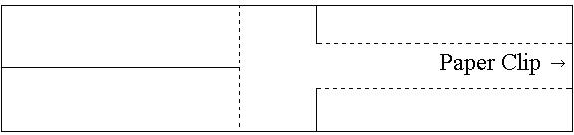
\includegraphics[width=0.4\textwidth]{./img/helicopter-1.png}
\end{center}

\begin{center}
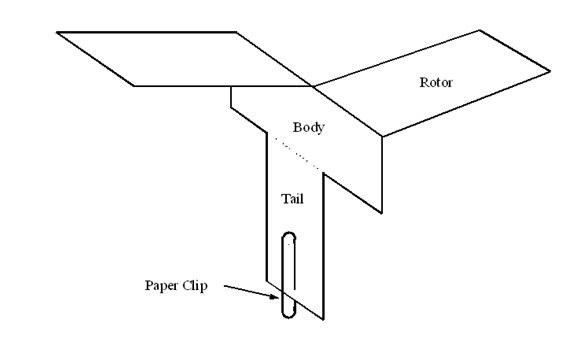
\includegraphics[width=0.4\textwidth]{./img/helicopter-2.png}
\end{center}

\begin{description*}
\item[Topic:]{Air Resistance (Force) - Form I}
\item[Materials:]{Paper, scissors, paper clip}
%\item[Setup:]{}
\item[Procedure:]{Copy the following design onto a piece of paper. Cut along the solid lines and fold along the dotted lines, attaching the paper clip to the bottom. Drop the helicopter with the paperclip down and watch it spin!}
%\item[Hazards:]{}
\item[Questions:]{Does the helicopter spin more if you add more paper clips? If you change the size/number of wings?}
\item[Observations:]{Adding more paper clips causes the helicopter to spin faster. Increasing the surface area of the wings also increases the rate of spin.}
\item[Theory:]{The helicopter spins because the force of air resistance pushing up on the wings creates a moment about the vertical axis of rotation. Increasing the force of air resistance thus increases this moment and hence the helicopter spins faster.}
%\item[Applications:]{}
%\item[Notes:]{}
\end{description*}

\subsection{Parachutes}

\begin{center}
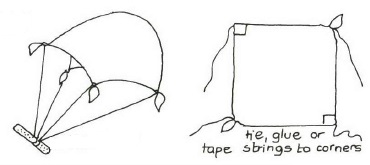
\includegraphics[width=0.4\textwidth]{./img/vso/parachute.png}
\end{center}

\begin{description*}
\item[Topic:]{Air Resistance (Force) - Form I}
\item[Materials:]{Paper/newspaper/plastic bags, string, paper clips}
\item[Setup:]{Tie pieces of string (about 30 cm) to each corner of the paper/bag. Join the four strings together and attach a paper clip or other small weight.}
\item[Procedure:]{Drop the parachute side by side with a normal paper clip.}
%\item[Hazards:]{}
\item[Questions:]{Which one reaches the ground first? If the paper clip were a person, which one would arrive safely to the ground? Does a person using a parachute want to make it as large as possible or as small as possible?}
\item[Observations:]{The parachute falls more slowly because there is a larger space for air to enter and counteract the force of gravity pulling it to the ground.}
%\item[Theory:]{}
\item[Applications:]{Skydivers, military personnel, air-dropped aid packages}
\item[Notes:]{Poke a small hole in the top of the parachute and ask students what will happen.}
\end{description*}

\subsection{Bucket Swing}

\begin{center}
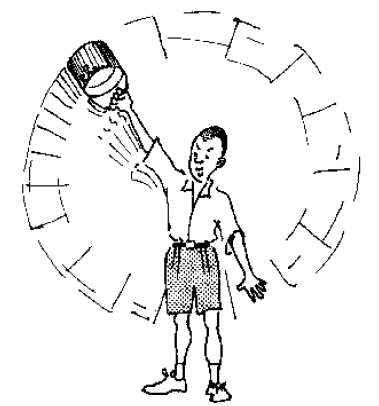
\includegraphics[width=0.4\textwidth]{./img/source/bucket-swing.png}
\end{center}

\begin{description*}
\item[Topic:]{Force - Form I}
\item[Materials:]{Bucket, rope, water}
%\item[Setup:]{}
\item[Procedure:]{Fill a bucket about half way with water and attach a rope to the handle. Swing the rope in a vertical circle so that the bucket is facing downwards at the top of its arc.}
\item[Hazards:]{Don't try to stop the bucket at the top of its swing.}
%\item[Questions:]{}
\item[Observations:]{The water remains in the bucket, even when turned upside-down. You can feel the bucket pulling outwards as you spin it.}
\item[Theory:]{The water and bucket are being pulled outwards by a force known as \emph{centripetal force}. This is essentially a result of the inertia of the items, as they want to continue their motion in a straight line path at any given point throughout the swing. You must constantly exert a force on the rope to cause the bucket to change its direction of motion.}
%\item[Applications:]{}
%\item[Notes:]{}
\end{description*}

\subsection{Egg Float}

\begin{center}
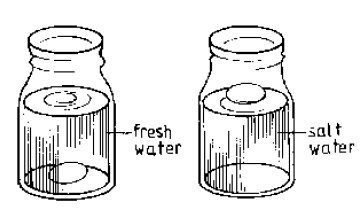
\includegraphics[width=0.4\textwidth]{./img/source/egg-float.png}
\end{center}

\begin{description*}
\item[Topic:]{Flotation - Form I}
\item[Materials:]{2 fresh eggs, 2 containers (bottles cut in half), salt (less than half a cup)}
\item[Setup:]{Fill the two containers with water and place a fresh egg in each.}
\item[Procedure:]{Leave one as it is and add salt to the other. Add and mix salt until the egg floats in the saltwater container.}
%\item[Hazards:]{}
\item[Questions:]{Why does the egg float in saltwater but sink in fresh water?}
%\item[Observations:]{}
\item[Theory:]{Saltwater has a greater density than fresh water. A fresh egg has a density between fresh water and saltwater. Since an egg is denser than freshwater, it sinks. Since an egg is less dense than saltwater, it floats.}
\item[Applications:]{This is the same reason why it is easier to stay afloat when swimming in the ocean (saltwater) as opposed to a lake (fresh water).}
%\item[Notes:]{}
\end{description*}

\vfill
\pagebreak

\subsection{Water Dome}

\begin{center}
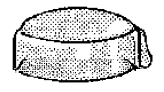
\includegraphics[width=0.2\textwidth]{./img/source/water-dome.png}
\end{center}

\begin{description*}
\item[Topic:]{Adhesion/Cohesion (Properties of Matter) - Form I}
\item[Materials:]{Coin, water, syringe or eyedropper}
%\item[Setup:]{}
\item[Procedure:]{Place the coin flat on a table. Use the syringe or eyedropper to carefully drop individual water drops onto the coin.}
%\item[Hazards:]{}
\item[Questions:]{How many drops do you think the coin can hold?}
\item[Observations:]{The coin holds a surprising number of drops and forms a dome shape before the water spills over.}
\item[Theory:]{The surface tension of the water holds it together against the force of gravity, which is trying to pull the water off the coin.}
%\item[Applications:]{}
%\item[Notes:]{}
\end{description*}

%\subsection{Exploring Adhesion and Cohesion}
%
%\begin{center}
%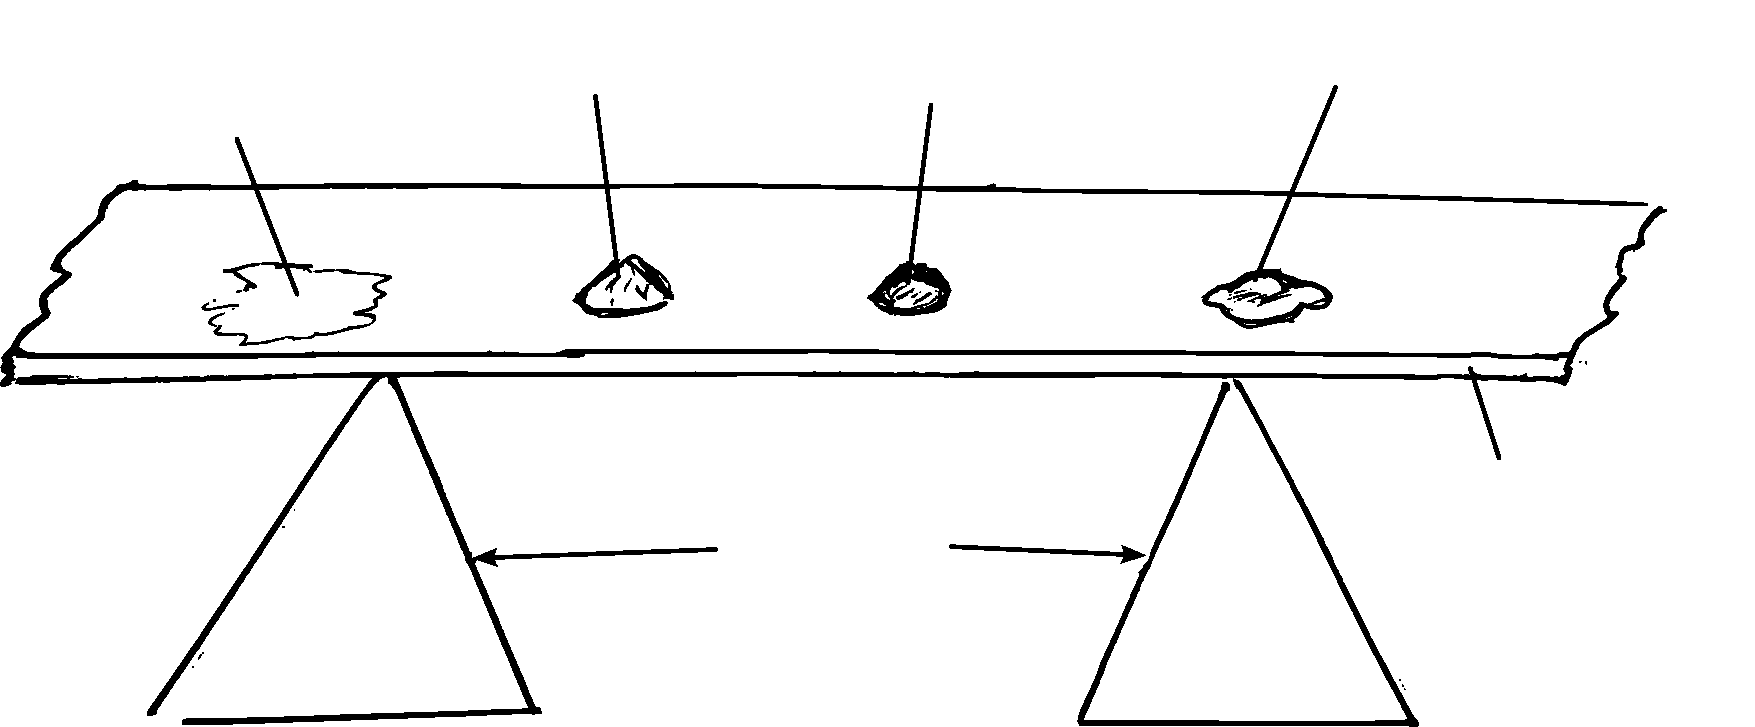
\includegraphics[width=0.4\textwidth]{./img/adhesion-cohesion.png}
%\end{center}
%
%\begin{description*}
%%\item[Subtopic:]{}
%\item[Materials:]{Sheet of glass, water, honey, glycerin, cooking oil, syringe, and 2 wooden blocks}
%%\item[Setup:]{}
%\item[Procedure:]{Place a sheet of glass over two wooden blocks on a table. Using a syringe, place a drop of different liquids on the glass.}
%%\item[Hazards:]{}
%%\item[Questions:]{}
%\item[Observations:]{Water spreads and wets the glass, while honey, glycerin and cooking oil remain in a spherical shape.}
%\item[Theory:]{The adhesive forces between the water molecules and glass molecules are greater, while the cohesive forces between the molecules of honey, glycerin and cooking oil are larger.}
%%\item[Applications:]{}
%%\item[Notes:]{}
%\end{description*}

\subsection{Pressure Increases with Depth}

\begin{center}
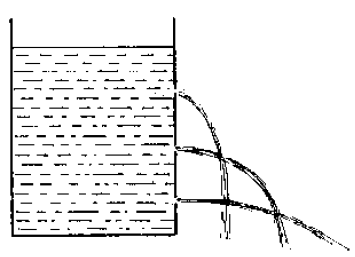
\includegraphics[width=0.3\textwidth]{./img/source/pressure-depth.png}
\end{center}

\begin{description*}
\item[Topic:]{Pressure - Form I}
\item[Materials:]{1.5 L bottle, syringe needle or pin/nail, water}
\item[Setup:]{Poke three holes into a bottle. Put one hole near the bottom, one near the middle, and the last hole between them.}
\item[Procedure:]{Fill the bottle with water and place on a table. Observe the trajectories of water coming from the three holes.}
%\item[Hazards:]{}
\item[Questions:]{Which stream goes the farthest distance horizontally? Which hole has the highest pressure?}
\item[Observations:]{The water flowing from the lower holes travels farther.}
\item[Theory:]{The added weight of the water above the lower holes increases the pressure there, resulting in an increased horizontal velocity. It is shown that pressure increases with depth ($P = \rho g h$).}
\item[Applications:]{The wall of a dam is made much thicker at the bottom than at the top. This is to reinforce against the increased water pressure at greater depths.}
%\item[Notes:]{}
\end{description*}

\subsection{Paper Jump}

\begin{center}
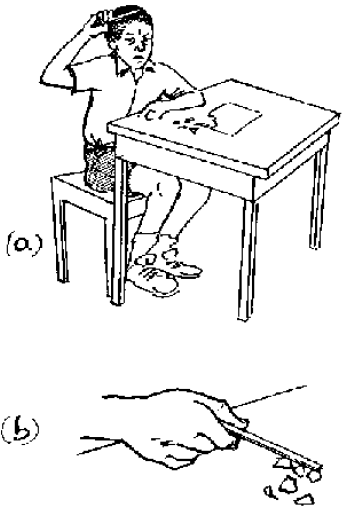
\includegraphics[width=0.3\textwidth]{./img/source/static-elec.png}
\end{center}

\begin{description*}
\item[Topic:]{Static Electricity - Form II}
\item[Materials:]{Small pieces of paper, ruler, pen, balloon, salt and pepper (optional)}
%\item[Setup:]{}
\item[Procedure:]{Rub a pen, ruler or blown up balloon against your hair for about 30 seconds. Then bring it close to the small papers on a table.}
%\item[Hazards:]{}
%\item[Questions:]{}
\item[Observations:]{The small papers jump and cling to the object.}
\item[Theory:]{When you rub the object against your hair, electrons are transferred by friction to the object, giving it a negative charge. When the negatively charged object approaches the papers, the electrons in the papers are repelled downwards and the protons are attracted towards the top. When the object is close enough the positive charges on the tops of the papers jump and cling to the negatively charged object.}
%\item[Applications:]{}
\item[Notes:]{Try also with salt and pepper. The pepper jumps but the salt is too heavy and does not.}
\end{description*}

\subsection{Conductors and Insulators}

\begin{center}
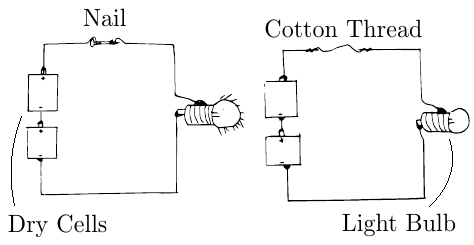
\includegraphics[width=0.49\textwidth]{./img/conductors-insulators.png}
\end{center}

\begin{description*}
\item[Topic:]{Current Electricity - Form II}
\item[Materials:]{Dry cells, light bulb, speaker wire, cardboard, various materials (nail, pen cap, aluminum foil, string, balloon, toothpick, bottle cap, pencil, etc.)}
\item[Setup:]{Connect the dry cells and light bulb using speaker wire and leave two ends of the wire free.}
\item[Procedure:]{Have students predict which materials will cause the bulb to light. Then try them one by one by placing across the free wire ends.}
%\item[Hazards:]{}
%\item[Questions:]{}
\item[Observations:]{Metal objects such as nails, aluminum foil, bottle caps, etc. turn on the light, while others do not.}
\item[Theory:]{Conductors are materials which allow electric current to pass through them easily, while insulators do not. Placing conducting materials (e.g. many metals) across the wires closes the circuit and allows electrons to flow through bulb and produce light.}
%\item[Applications:]{}
%\item[Notes:]{}
\end{description*}

\subsection{Magnetic Filings}

\begin{center}
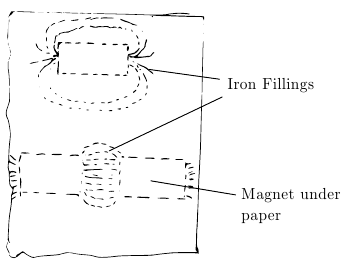
\includegraphics[width=0.4\textwidth]{./img/magnetic-fields.png}
\end{center}

\begin{description*}
\item[Topic:]{Magnetism - Form II}
\item[Materials:]{Bar magnets, paper, steel wool}
%\item[Setup:]{}
\item[Procedure:]{Place one or two bar magnets under a sheet of paper. Sprinkle iron filings over the top to reveal the lines of the magnetic field.}
%\item[Hazards:]{}
%\item[Questions:]{}
\item[Observations:]{The iron filings reveal the magnetic lines of force.}
\item[Theory:]{Filings gather around the poles, where the magnetic force is strongest. Lines of repulsion are seen for like poles, and there is a \emph{neutral point} in the center through which no lines pass. Lines of attraction are shown for unlike poles.}
%\item[Applications:]{}
%\item[Notes:]{}
\end{description*}

\subsection{Electromagnet}

\begin{center}
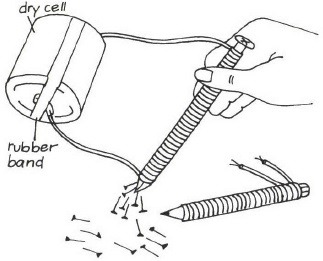
\includegraphics[width=0.4\textwidth]{./img/vso/electromagnet.png}
\end{center}

\begin{description*}
\item[Topic:]{Magnetism - Form II}
\item[Materials:]{Dry cell, nail, insulated copper wire, pins}
%\item[Setup:]{}
\item[Procedure:]{Make about 50 turns of wire around the nail. Connect the wire to the dry cell. Pick up the pins with the magnetised nail.}
%\item[Hazards:]{}
%\item[Questions:]{}
%\item[Observations:]{}
\item[Theory:]{The nail is magnetised by the electrical method. The moving electric charge in the wire solenoid creates a magnetic field in the nail. The stronger the current and the greater the number of turns of wire, the stronger the magnet.}
%\item[Applications:]{}
%\item[Notes:]{}
\end{description*}

\end{multicols}